\subsubsection{Pre-Join procedure}
The Pre-Join procedure is a necessary step to give to PIVOT an initial view about which EDs are currently operating in the network. Indeed, when the system is turned on and start receiving packets, it has no historical trace of the devices in the network, either of the messages they sent before its activation. This implies that the vector \(\ C \) is initially \textit{empty} and therefore, there are no saved pattern to use in the matching process. Then, the Pre-Join procedure is a initial step through which the first patterns are identified and modeled. They will subsequently be used as a reference in the \textit{Main} procedure.

\vspace{5mm}

In detail, for each packet \(\ p \) received in input, the algorithm reads the DevAddress \(\ a \) and the timestamp \(\ t \). There are two scenarios:

\vspace{3mm}
\begin{enumerate}
	\item \(\ P_{a} \notin  C\). A new pattern \(\ P_{a} \) is \textit{initialized}.
	\item \(\ P_{a} \in C\). The pattern \(\ P_{a} \) is \textit{updated}
\end{enumerate}
\vspace{3mm}

According to the Section \ref{updating}, the initialization of a new pattern consists in the creation of an empty chain \(\ P_{a} = \{\} \) to store together with the DevAddress \(\ a \), the timestamp \(\ t \) and the flag \(\ verified \), set to \textit{False}. In the same way, updating an existing pattern implies calculating the \textit{current} segment \(\ t - t_{f} \) and checking if \(\ s \) is already in the chain.

\vspace{4mm}
\begin{algorithm}
    \caption{Pre-Join procedure}
    \begin{algorithmic}[1]
        \If{$a$ in $C$}
            \State $P \gets C(a)$
            \State $P.update(t)$
        \Else
            \State $P \gets newPattern(a)$
            \State $C(a) \gets P$
        \EndIf
    \end{algorithmic}
\end{algorithm}
\vspace{4mm}

The Pre-Join terminates when PIVOT receives as input the first Join-request. At the end of this phase, the number of DevAddress \(\ a_{1}, a_{2}, ..., a_{n} \) collected matches with the number of devices that sent messages \(\ ED_{1}, ED_{2}, ..., ED_{n} \). According to the LoRaWAN specification, a device \(\ ED_{i} \) modifies the DevAddress \(\ a_{i} \) only when it disconnects from the network and performs an new OOTA. This step ends exactly at the moment the first Join-request arrives. Then, for the entire duration of the Pre-Join procedure there is no \(\ ED \) that changes the associated DevAddress. All the pattern detected and stored in the vector \(\ C \) are in a \textit{one-to-one} relationship with all the collected DevAddress.

\vspace{5mm}

As we have seen, a variable that determines the temporal window of the Pre-Join is the instant in which a device sends a Join-request. It is an uncertain and unpredictable phenomenon that can affect the accuracy of the detected patterns of \(\ C \). Indeed, if the period \(\ \tau \) of a pattern is longer than the duration of the procedure, the algorithm cannot correctly estimate all the segments that make up the chain. The flag \textit{verified} is designed precisely to indicate the completeness of a pattern. Let \(\ V \) the list of patterns with the flag \textit{verified = True}, then \(\ V \subseteq C\). In the best case, at the end of the Pre-Join, the patterns in the vector \(\ C  \) are all complete, allowing the detection algorithm to perform more precise matches.

\vspace{3mm}
\begin{figure}
    \centering
    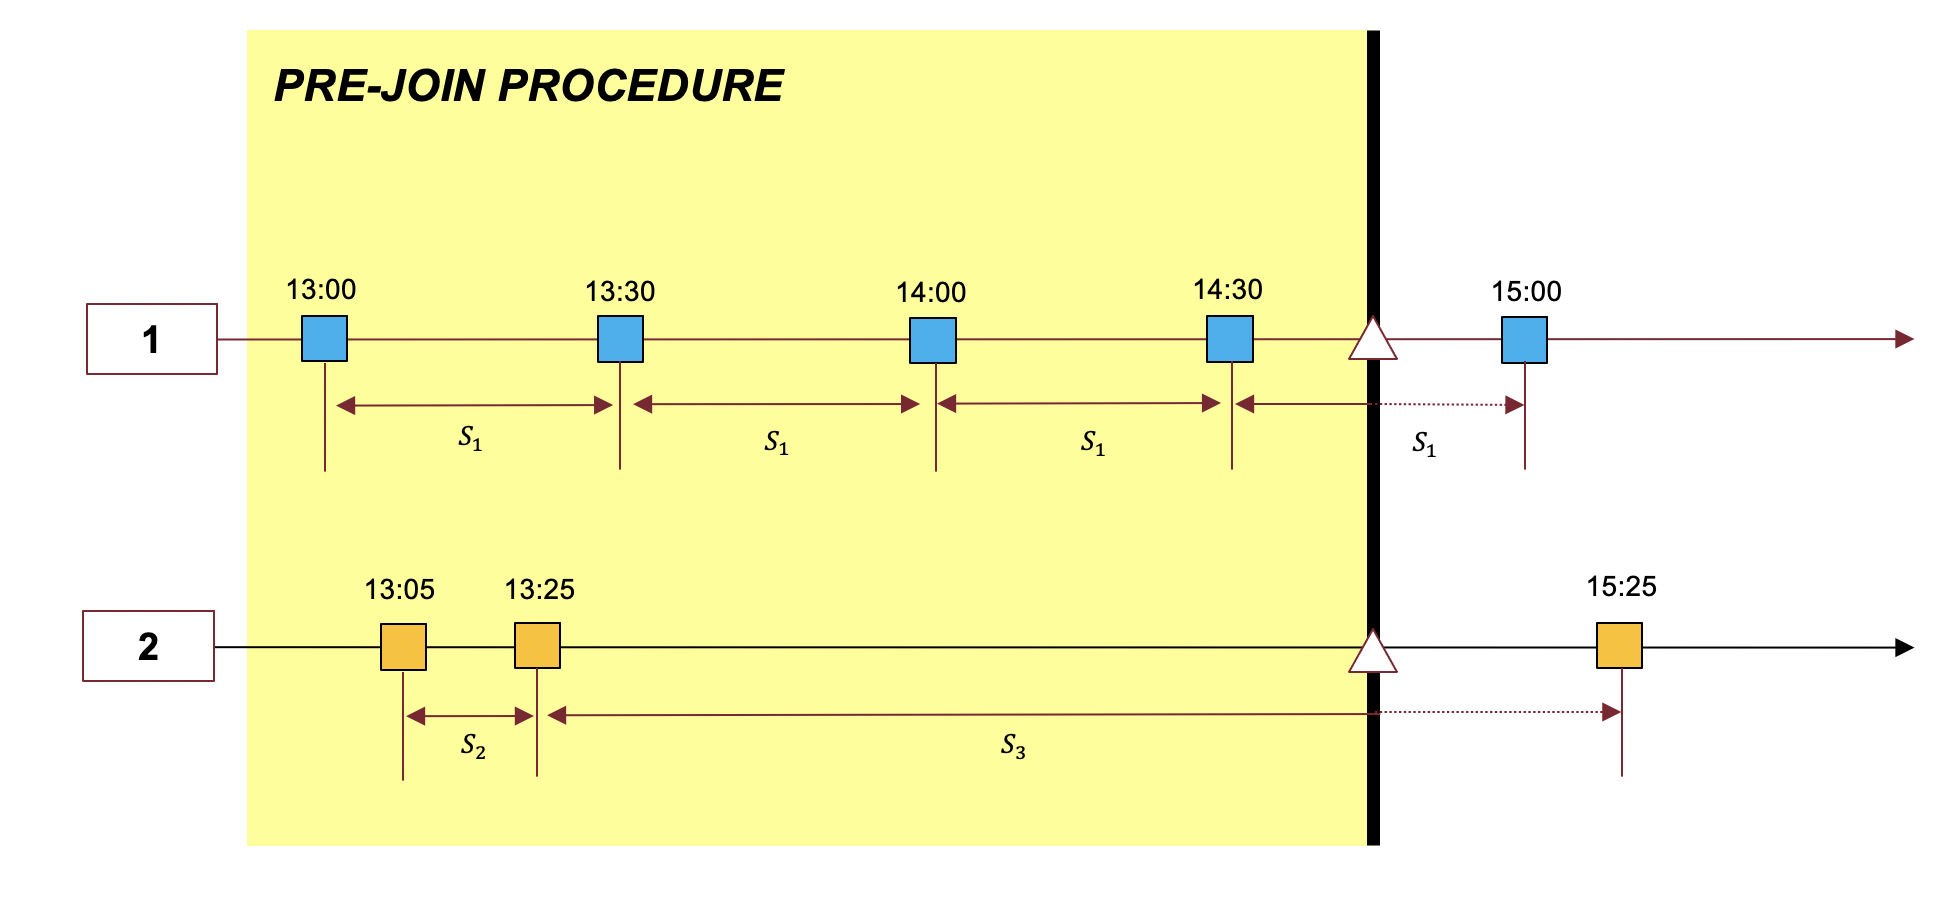
\includegraphics[width=0.7\linewidth]{images/pivot/missing_pattern.png}
    \caption{An example of pattern with different periods \(\ \tau_{1} = 0.5 \) and \(\ \tau_{2} = 2.3 \). At the end of the Pre-Join procedure, only the first pattern is recognized.}
\label{fig:missing}
\end{figure}
\vspace{3mm}

The example reported in figure \ref{fig:missing} shows two different patterns \(\ P_{1} = \{ s_{1} \} \) and \(\ P_{2} = \{ s_{2}, s_{3} \} \), where \(\ s_{1} = 0.5 \), \(\ s_{2} = 0.33 \) and \(\ s_{3} = 2.0 \). If the duration of the Pre-Join procedure is an hour and three quarters (or \textit{1.75}), the algorithm can't determine all the segments that composes the chain of \(\ P_{2} \). Then to \(\ P_{2} \) is associated the flag \textit{verified = False}. On the contrary, since \(\ P_{1} \) has a smaller period \(\ \tau = 0.5\),  is correctly recognized, the flag \textit{verified} of \(\ P_{1} \) is set to True.
\vspace{5mm}